% !TeX spellcheck = en_GB
\documentclass[10pt,letterpaper,oneside]{article}
\usepackage{fontspec}
\usepackage{arev}
\usepackage[utf8]{inputenc}
\usepackage[T1]{fontenc}
\usepackage{amsmath}
\usepackage{amsfonts}
\usepackage{amssymb}
\usepackage{graphicx}
\usepackage{csquotes}
\usepackage{booktabs}
\usepackage{multicol}
\usepackage{enumerate}
\usepackage{microtype}
\usepackage[labelfont=bf,font={small}]{caption}
\usepackage{hyperref}
\usepackage{booktabs}
\usepackage{subcaption}
\usepackage{fancyhdr}
\usepackage[svgnames]{xcolor}
\usepackage{mdframed}
\usepackage{multicol}
\usepackage[para]{footmisc}
\usepackage{siunitx}
\usepackage{cleveref}
\usepackage{listings}
\usepackage{cprotect}


\lstset{ % General setup for the package
	language=Python,
	basicstyle=\small\ttfamily,
	tabsize=4,
	columns=fixed,
	showstringspaces=false,
	showtabs=false,
	keepspaces,
	commentstyle=\color{SeaGreen},
	keywordstyle=\bf\ttfamily\color{DarkBlue}
}

\newfontfamily\symbolfont{Symbola}
\usepackage[left=1in,right=1in,top=1in,bottom=1in,marginparwidth=0.3in]{geometry}

\usepackage[sorting=none]{biblatex}
\addbibresource{../bibliography.bib}

\author{Andreas Stöckel\\[0.5cm]Based on lecture notes by\\Chris Eliasmith and Terrence~C.~Stewart}
\newcommand{\baseCodeURL}{https://github.com/astoeckel/syde556-w20/blob/master/lectures}

\fancyhf{}
\fancyhead[L]{SYDE 556/750 Lecture Notes}
\fancyhead[R]{Andreas Stöckel}
\fancyfoot[C]{\thepage}
\pagestyle{fancy}

\setlength{\parindent}{0em}
\setlength{\parskip}{0.5em}
\renewcommand{\baselinestretch}{1.25}
\renewcommand{\vec}[1]{{\mathbf{#1}}}
\newcommand{\mat}[1]{{\mathbf{#1}}}
\newcommand{\T}{\ensuremath{\mathrm{T}}}
\renewcommand{\epsilon}{\varepsilon}
\renewcommand{\phi}{\varphi}

\makeatletter
\newcommand{\superimpose}[2]{%
	{\ooalign{{#1}\hidewidth\cr{#2}\hidewidth\cr}}}
\makeatother
\newcommand{\SolidCircle}[2]{\superimpose{\color{#1}\symbolfont ⬤}{\textbf{\color{white}#2}}\hspace{1em}}
\newcommand{\OPlus}{\SolidCircle{DarkGreen}{\kern0.75pt+}}
\newcommand{\OMeh}{\SolidCircle{DarkOrange}{~}}
\newcommand{\OMinus}{\SolidCircle{DarkRed}{\kern2.25pt--}}

\newcommand{\YouTube}[2][Video]{\href{https://youtu.be/#2}{{\symbolfont 📺}~{#1}}%
%\footnote{\url{https://youtu.be/#2}}%
}

\newcommand{\CodeLink}[2][Code]{\href{\baseCodeURL/#2}{{\symbolfont ⌨}~\emph{#1}}}

\newcommand{\MakeTitle}[1]{
\maketitle
\begin{center}
	
\includegraphics[width=0.5\textwidth]{../assets/uwlogo.pdf}\\[1cm]
	{#1}\
\end{center}

\vfill

\thispagestyle{empty}
\setcounter{page}{0}
\newpage

\pagenumbering{roman}
\setcounter{tocdepth}{2}
\tableofcontents
\newpage

\setcounter{page}{0}
\pagenumbering{arabic}}

\reversemarginpar


\newcommand{\ColorBox}[3]{%
	\marginpar{%
		\huge\raisebox{-3ex}{\symbolfont{#1}}%
	}%
	\begin{mdframed}[hidealllines=true,backgroundcolor=#2,innertopmargin=0.25cm,innerbottommargin=0.25cm]%
		{#3}
	\end{mdframed}}

\newcommand{\Note}[1]{\ColorBox{📌}{WhiteSmoke}{\textbf{Note:} #1}}
\newcommand{\Example}[1]{\ColorBox{💡}{WhiteSmoke}{\textbf{Example:} #1}}
\newcommand{\Aside}[1]{\ColorBox{🌟}{WhiteSmoke}{\emph{Aside:} #1}}
\newcommand{\Python}[1]{\ColorBox{🐍}{WhiteSmoke}{#1}}
\newcommand{\Notation}[1]{\ColorBox{\huge$\Sigma$}{WhiteSmoke}{\textbf{Notaton:} #1}}

\newcommand{\ConstructionSite}{\hrulefill {\symbolfont 🚧} UNDER CONSTRUCTION {\symbolfont 🚧} \hrulefill}

\newenvironment{ImportantEqn}[1]{\mdframed\raggedleft\emph{({#1})}\align}{\endalign\endmdframed}

\date{January 23 \& 28, 2020}
\title{SYDE 556/750 \\ Simulating Neurobiological Systems \\ Lecture 4: Temporal Representation}


\begin{document}

\MakeTitle{\textbf{Accompanying Readings: Chapter 4 of Neural Engineering}}

\section{Introduction}

\Note{We set out to build a theory describing what \enquote{the neural code} may be. In Lecture~2 we discussed individual neuron models, and roughly modelled their behaviour in terms of a rate approximation $G[J]$. We continued in Lecture 3 to think about \enquote{representation} in groups of neurons, i.e.,~what the \emph{activity} of individual neurons represents in terms of (external) stimuli. While this brings us closer to a theory of the \enquote{neural code}, one important notion has been missing so far: time.}

We discussed how neural populations could be modelled as representing vectorial quantities. In particular, we assumed that each neuron in a population essentially computes a spike rate $G[J]$ in spikes per second, given an input current $J$. As we saw when we were discussing the LIF neuron model, this is not the case in biology. Neurons are dynamical systems that receive stimuli over time and output a sequence of spikes.

The output of a biologically plausible neuron model is also called a \emph{spike train}. Given an input current over time, the $i$-th neuron in a neural population produces a series of output spikes at time points $t^1_i, t^2_i, \ldots$, and so on. We model a spike train as a continuous function over time by superimposing a set of Dirac-$\delta$ functions
\begin{align*}
	a_i(t) &= \sum_{k = 1}^\infty \delta\big(t - t^k_i\big) \,.
\end{align*}

\Note{As detailed in the notes for Lecture 2, the Dirac-$\delta$ function is defined as the function $\delta(t)$ that is zero for all points $t \neq 0$, but has a definite integral from $-\infty$ to $\infty$ of one.}

As before, our goal is to decode (\enquote{read out}) the value represented in the neural population. However, in contrast to what we did before, we would like to decode the value represented in the population at \emph{any time} $t$. We will solve this problem in three steps: first, we explore what happens if we use exactly the same technique we used before on the spike trains produced by a neural population. Then, we try to remove noise in the estimate by computing an optimal filter. Lastly, we consider what the biological correlate of such a filter could be.

\section{Solving for a Spike Train Decoder}

Our first attempt at decoding a neural representation is similar to what we did before -- we gather a bunch of training data, consisting of a time-series of neural activity $\vec a(t)$ and a represented value $\vec x(t)$. We arrange discrete samples of these activities in matrices $\mat A$ and $\mat X$ and compute a decoder $\mat D$. Then, we can decode the represented value according to the decoding equation $\hat{\vec x}(t) = \mat D \vec a(t)$.


\subsection{Discretizing Spike Trains}

In the previous lecture, we discussed computing a decoder $\mat D$ by choosing a random set of $N$ samples $\big\{ \vec x_1, \ldots, \vec x_N \big\} \subset \mathbb{X}$, forming a matrix $\mat X \in \mathbb{R}^{d \times N}$, as well as recording the associated nonnegative population activities $\big\{ \vec a(\vec x_1), \ldots, \vec a(\vec x_N) \big\} \subset \mathbb{R}^n$, forming a matrix $\mat A \in \mathbb{R}^{n \times N}$, where $n$ is the number of neurons in the population.

Now, the question is how to gather such training data in the time-continuous case. One procedure that could accomplish this is to generate a random signal, $\vec x(t)$, feeding this signal into the neuron population, and recording the neural activities. In other words, for each neuron~$i$ in the population, we have the encoding equation
\begin{align*}
J_i(t) &= \alpha_i \langle \vec e_i, \vec x(t) \rangle + J^\mathrm{bias}_i \,, \\
a_i(t) &= \sum_{k=1}^\infty \delta\big(t - t^k_i\big) \,,
\end{align*}
where $t^k_i$ is the time of the $i$-th spike produced by our neuron model for an input current $J_i(t)$. In case we chose the LIF neuron model, we would for example use $J_i(t)$ as an input in the following sub-threshold differential equation
\begin{align*}
\frac{\mathrm{d}}{\mathrm{d}t} v_i(t) &= -\frac{1}{\tau_\mathrm{RC}} \big( v_i(t) - J_i(t) \big) \,, \quad &\text{if } v_i(t) &< 1\,,
\end{align*}
with the appropriate super-threshold behaviour following spike production -- whenever $v_i(t)$ reaches the threshold potential $v_\mathrm{th} = 1$ (assume that this happens at a time $t_i^k$, where $k$ is an incrementing spike index), we clamp the membrane potential to the reset potential $v_\mathrm{reset} = 0$ for $\tau_\mathrm{ref}$ seconds
\begin{align*}
v(t) &\gets 0 \,, &\text{if } t &> t_i^k \text{ and } t \geq t_i^k + \tau_\mathrm{ref} \,, \text{for all spike times } t_i^k \,.
\end{align*}
To summarize, we have two time-continuous functions: $\vec x(t)$, our randomly created input function, and $\vec a(t)$, the spike trains produced by our neurons for the given represented values.

Now, how do we assemble our matrices $\mat X$ and $\mat A$? Note that we have described $\vec x(t)$ and $\vec a(t)$ in continuous time, yet these matrices need to be constructed out of $N$ discrete values. The answer is that we simply discretise our function into short time-slices of width $\Delta t$, starting at a time zero, and stopping at a time~$T$. We then have $N = \lfloor T / \Delta t \rfloor$ time slices, and each of these time slices can be interpreted as one of $N$ samples for our matrix.

\Note{\emph{Discrete Dirac-$\delta$.} We discuss generating a discrete random input function $\vec x(t)$ below. However, it is unclear how to discretise the population response $\vec a(t)$, since each individual neural response $a_i(t)$ is a sum of Dirac-$\delta$ functions. Luckily, this can be easily resolved by recalling the two important properties of the Dirac-$\delta$ listed above: being zero at all except for one point, and the integral being one. If we want to retain these properties in the discrete case, this means that the Dirac-$\delta$ is zero for all sample points except for one sample point which we have to set to $\Delta t^{-1}$ to get an area-under-the-curve of one when we discretise the integral. Assuming we have a spike at time $t'$ with $0 < t' < T$, we get
\begin{align*}
	\int_{0}^T \delta(t - t') \,\mathrm{d}t &= \sum_{i = 1}^N f_i \Delta t = \frac{\Delta t}{\Delta t} = 1 \,, &\text{where } f_i &=
	\begin{cases}
		\frac{1}{\Delta t} & \text{if } i \neq \left\lfloor\frac{t'}{\Delta t}\right\rfloor \,,\\
		0 & \text{otherwise} \,, \\
	\end{cases}
\end{align*}
where $f_i$ are the discrete samples of the function.
}

\subsection{Random Signals}

\begin{figure}
	\centering
	\begin{subfigure}{\textwidth}
		\centering
		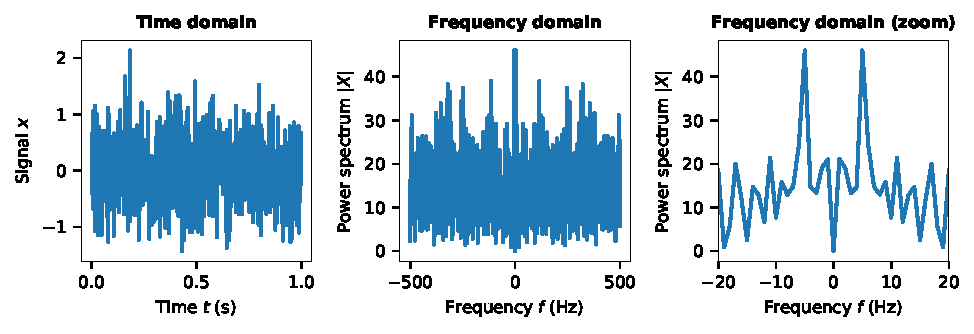
\includegraphics{media/white_noise.pdf}
		\caption{Zero mean white white noise}
		\label{fig:white_noise}
	\end{subfigure}
	\begin{subfigure}{\textwidth}
		\centering
		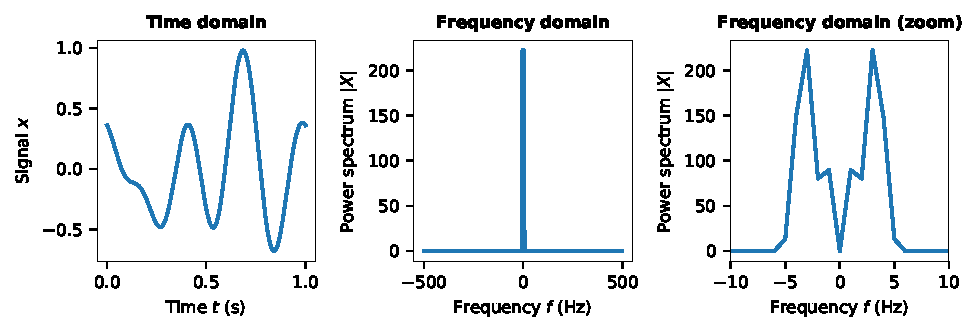
\includegraphics{media/white_noise_5hz.pdf}
		\caption{Zero mean \SI{5}{\hertz} bandlimited white noise}
		\label{fig:white_noise_5hz}
	\end{subfigure}
	\caption{Comparison between white noise and bandlimited white noise. Discrete signals generated with a time step of $\Delta t = \SI{1}{\milli\second}$. \CodeLink{lecture_04/media/code/filter_examples.ipynb}}
\end{figure}

We mentioned above that we would like to randomly generate an input function $x(t)$. But what exactly do we mean by random? And how do we turn such a function into discrete time steps? A somewhat na\" ive attempt would be to select a timestep $\Delta t$, a maximum time $T$, and to just sample $N = \lfloor T / \Delta t \rfloor$ values from a Gaussian distribution. This kind of noise, where the individual points in time are independently sampled from a Gaussian distribution is called \emph{white noise}.

\Cref{fig:white_noise} shows what such a signal would look like for a time step $\Delta t = \SI{1}{\milli\second}$ and $T = 1$. Interestingly, the signal looks -- qualitatively -- the same in both the time and the frequency domain. Instead of generating this kind of signal in the time domain we could also create it in the frequency domain by generating random complex numbers for each Fourier coefficient
\begin{align*}
	x(t) \sim \mathcal{N}(0, 1) \Leftrightarrow X(\omega) = X(-\omega) = a + ib \text{, where } a \sim \mathcal{N}(0, 1) \text{ and } b \sim \mathcal{N}(0, 1) \,,
\end{align*}
where $X = \mathcal{F}[x]$ is Fourier-transformed signal. In particular, $X(\omega)$ is a function over the angular frequency $\omega = 2\pi f$.

It is impossible to generate true white noise (i.e.,~as $\Delta t \to 0$) in a physical system, since even finite portions of the signal contain an infinite amount of energy (remember that signal must change instantaneously between individual \enquote{quanta} of time). But even less fundamentally, we find that signals in the physical world are usually quite \emph{smooth} -- there are no sudden changes between values.

Hence, to model physical stimuli we may want to use \emph{bandlimited white noise} -- that is, we have some upper frequency $\hat f$ above which all frequency coefficients are zero. We can easily generate such a signal $x(t)$ by applying our above observation, namely that white noise in the time domain looking the same as in the frequency domain: we simply sample a set of complex numbers $z_1, \ldots, z_d$ corresponding (indirectly, see note) to the phases and powers of frequencies up to $\hat f$. We then apply the inverse Discrete Fourier Transformation (DFT) and voilà, we get our band-limited white noise function in the time domain $x(t)$ (\cref{fig:white_noise_5hz}). For a $d$-dimensional $\vec x(t)$ we simply repeat this process $d$ times.

\Note{\emph{Fourier Transformation.} The Fourier transformation decomposes a signal $x(t)$ into a sum of phase-shifted sine waves of different frequencies. Fourier's insight was that any (complex-valued) function $x(t)$ can be decomposed into an infinite sum of sine and cosine waves. It holds
	\begin{align*}
	X(\omega) = \mathcal{F}[x](\omega) = \int_{-\infty}^{\infty} x(t) e^{-i t \omega} \, \mathrm{d}t = \int_{-\infty}^{\infty} x(t) \left[ \cos(-t\omega) - i \sin(t\omega) \right] \mathrm{d}t\,.
	\end{align*}
	Intuitively, for a fixed angular frequency $\omega$, this function can be interpreted as computing the \enquote{similarity} (in terms of an inner product over functions) between the function $x(t)$ and the periodic signals $\cos(-t\omega)$ and $\sin(t\omega)$. Consider a specific value $X(\omega) = z = a + ib$, where $a$ is the \enquote{real} value of the complex number $z$ and $b$ is the \enquote{imaginary} part of $z$. The similarity with the cosine is stored in $a$, the similarity with the sine is stored in $b$.

	The \emph{power}, or \enquote{magnitude}, of a particular frequency $\omega$ is given as $|z| = \sqrt{a^2 + b^2}$. The complex coefficients $a$ and $b$ also encode the \emph{phase} $\phi$ of that particular frequency, where $\phi = \mathrm{arctan2}(b, a)$.

	\emph{Inverse Fourier Transformation.}
	The Fourier transformation can be inverted by applying almost the same transformation again (note the flipped sign in the exponential):
	\begin{align*}
		x(t) = \mathcal{F}^{-1}[X](t) = \int_{-\infty}^{\infty} X(\omega) e^{i t \omega} \, \mathrm{d}\omega = \int_{-\infty}^{\infty} X(\omega) \left[ \cos(t\omega) +¸ i \sin(t\omega) \right] \mathrm{d}\omega\,.
	\end{align*}
}
\newpage

\Note{\emph{Properties of the Fourier Transformation.}
	\begin{itemize}
		\item The Fourier Transformation is \emph{linear}. In other words, it holds
		\begin{align*}
		 	\mathcal{F}[a f + b g] = a \mathcal{F}[f] + b \mathcal{F}[g] \,,
		\end{align*}
		where $a$, $b$ are scalars and $f$, $g$ are arbitrary functions over time.

		\item It holds $X(\omega) = X(-\omega)$ exactly if $x(t)$ is a purely real valued signal. In other words, to ensure that the inverse Fourier Transformation outputs a real-valued signal we must choose $X(\omega)$ to be symmetric.
	\end{itemize}
}


\cprotect\Python{\emph{Discrete Fourier Transformation.}
	We can write the above integral as a sum for discrete signals $x_0, \ldots, x_{N - 1}$. We get
	\begin{align*}
		X_i &= \sum_{k = 0}^{N - 1} x_k e^{-i \frac{i 2 \pi}{N} kn} \,,
	\end{align*}
	the so called Discrete Fourier Transform (DFT). You can compute the DFT of a signal $\vec x = (x_0, \ldots, x_{N - 1})$ in Python using the following code (see this \CodeLink[this Jupyter notebook]{lecture_04/media/code/dft_numpy_experiments.ipynb}).
	\begin{lstlisting}[language=python]
import numpy as np
dt = 1e-3                  # One millisecond time step
T  = 10.0                  # Maximum time: 10 seconds
ts = np.arange(0, T, dt)   # Sample points
N  = ts.size               # Number of samples

# Generate a one Hertz sine wave
f  = lambda t: np.sin(2 * np.pi * t) 
xs = f(ts)                 # Sample some function over time

# Compute the Discrete Fourier Transform using a fast algorithm
# called the "Fast Fourier Transformation" (FFT)
Xs = np.fft.fftshift(np.fft.fft(xs))

# Compute the frequency corresponding to each coefficient
fs = np.fft.fftshift(np.fft.fftfreq(N, dt))

# Reconstruct the original signal, throw away residual imaginary coefficients
xs_hat = np.real(np.fft.ifft(np.fft.ifftshift(Xs)))
\end{lstlisting}
The function \texttt{fftshift} arranges the Fourier coefficients such that the $k$-th coefficient $X_k$ corresponds to the frequency $\frac{2k - N}{2T} = \frac{2k - N}{2 \Delta t N}$ (for even $N$). \texttt{ifftshift} is the inverse of \texttt{fftshift}.
}

\newpage

\Aside{
	Have a look at the following resources if you would like to learn more about the Fourier transformation:
	\begin{itemize}
		\item Two videos by Grant Sanderson (3Blue1Brown) on the Fourier transformation:
		\begin{itemize}
			\item \YouTube[But what is the Fourier Transform? A visual introduction.]{spUNpyF58BY}
			\item \YouTube[But what is a Fourier series? From heat flow to circle drawings.]{r6sGWTCMz2k}
		\end{itemize}
		\item An Interactive Introduction to Fourier Transforms
by Jez Swanson:\\\url{http://www.jezzamon.com/fourier/index.html}
		\item Primer on the Discrete Fourier Transformation in the context of signal processing:\\\url{https://jackschaedler.github.io/circles-sines-signals/part3.html}
	\end{itemize}
}

\subsection{Computing Decoders}

\begin{figure}[p]
	\begin{subfigure}[b]{0.4\textwidth}
		\centering
		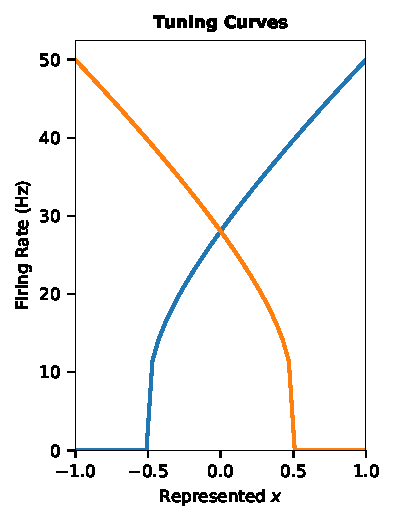
\includegraphics{media/two_neurons_tuning_curves.pdf}
		\caption{Population Tuning}
	\end{subfigure}
	\begin{subfigure}[b]{0.6\textwidth}
		\centering
		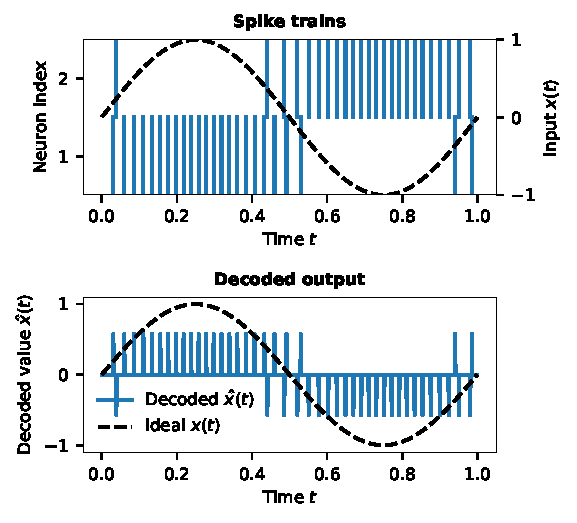
\includegraphics{media/two_neurons_spike_train.pdf}
		\caption{Spike Trains and Decoding}
	\end{subfigure}
	\caption{\textbf{(a)} Neural population tuning curves for two neuron. \textbf{(b)} Recorded spike trains for a sine-wave input (\emph{top}) and decoded output (\emph{bottom}). Time step of $\Delta t = \SI{1}{\milli\second}$. \CodeLink{lecture_04/media/code/time_continuous_decoding_experiment.ipynb}}
	\label{fig:two_neurons}
\end{figure}

\begin{figure}[p]
	\begin{subfigure}[b]{0.4\textwidth}
		\centering
		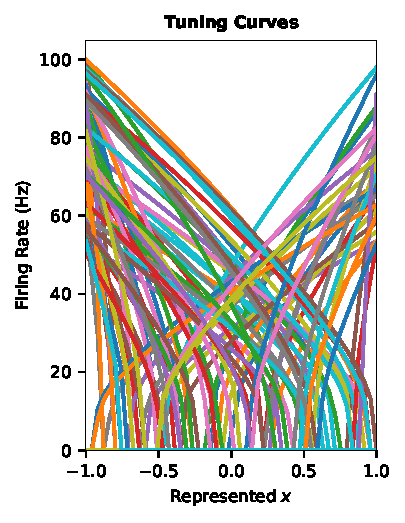
\includegraphics{media/hundred_neurons_tuning_curves.pdf}
		\caption{Population Tuning}
	\end{subfigure}
	\begin{subfigure}[b]{0.6\textwidth}
		\centering
		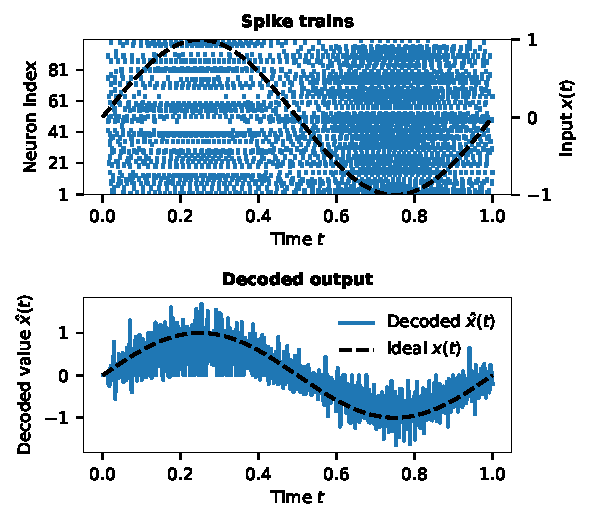
\includegraphics{media/hundred_neurons_spike_train.pdf}
		\caption{Spike Trains and Decoding}
	\end{subfigure}
	\caption{\textbf{(a)} Neural population tuning curves for one hundred neurons. \textbf{(b)} Recorded spike trains for a sine-wave input (\emph{top}) and decoded output (\emph{bottom}).  Time step of $\Delta t = \SI{1}{\milli\second}$. \CodeLink{lecture_04/media/code/time_continuous_decoding_experiment.ipynb}}
	\label{fig:hundred_neurons}
\end{figure}

Given a discretised version of our input function $\vec x(t)$ and the recorded population spike trains $\vec a(t)$, we can finally construct matrices $\mat X$ and $\mat A$ and use these to compute a set of decoders $\mat D$ according to the least-squares solution we discussed in the last lecture
\begin{align*}
	\mat D^\T &= (\mat A \mat A^\T)^{-1} \mat A^\T \mat X \,.
\end{align*}
Note that it is not necessary to use the regularised version of this equation. As we discussed last lecture, regularisation is not necessary in case we have a large number of noisy samples -- which is exactly what we have in this case. For example, if we record neural activities for a few neurons over $T = \SI{10}{\second}$ at a time step of $\Delta t = \SI{1}{\milli\second}$ we already have \num{10000} samples for each neuron.

\Note{\emph{Interpretation of the decoder computation equation.} If we were to analyse the above equation more thoroughly, we see that we are implicitly approximating the average firing rate for each neuron, given a certain input $\vec x$.
	
In a sense, we are computing the rate approximation $G[J]$ of the individual neurons \enquote{on the fly}. This has the consequence that our decoders $\mat D$ computed using the rate approximation $G[J]$ should still work in a spiking context. However, one advantage of this way of computing decoders is that it also works for more complicated neuron models for which we cannot easily compute a rate approximation $G[J]$.}

\paragraph{Example: Decoding from two neurons}
\Cref{fig:two_neurons} shows an example of what we have discussed above. In this particular case, we choose neural parameters $e_i$, $\alpha_i$, $J^\mathrm{bias}_i$ such that we have one neuron approximately covering the positive space of represented values, and another neuron covering the negative space of represented values. The decoder $\vec d$ for these two neurons is approximately
\begin{align*}
	\vec d = \begin{pmatrix} 0.5 \Delta t, & -0.5 \Delta t \end{pmatrix} \,.
\end{align*}
Whenever we receive a spike from the first neuron (each spike modelled as a discrete Dirac-pulse of height $1/\Delta t$) we decode out $0.5$, whenever we receive a spike from the second neuron we decode out $-0.5$. We do not have any information \enquote{in between spikes}.

\paragraph{Example: Decoding from one hundred neurons}
If we increase the number of neurons, the chance of multiple neurons spiking in the same timestep increases. In this case, our decoded output actually starts to look more like what we would expect (\cref{fig:hundred_neurons}) -- in particular, since there is a smaller change of being \enquote{in between spikes}, the decoded output does not constantly return to zero. Unfortunately, this is solely an artefact of discretisation. As we decrease our timestep $\Delta t$, it gets less and less likely for two neurons to be spiking in exactly the same timestep.


\section{Temporal Filtering}

Our method of computing decoders seems to work, however, we have the general problem that we have no data whenever there is no spike, which is particularly problematic if we let $\Delta t \to 0$. As we decrease the time step, it will be less likely that multiple $\delta$-functions coincide. One solution to this problem is to apply a temporal filter to our decoded signal that fills in values between individual spikes, or, if we regard the signal as a \enquote{noisy} version of the original signal, eliminates the noise.

\subsection{Gaussian Filters}

\begin{figure}
	\centering
	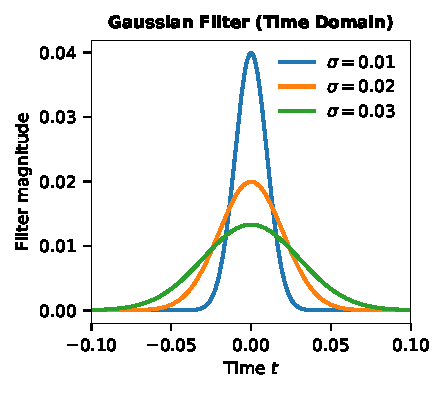
\includegraphics{media/gaussian_filters.pdf}
	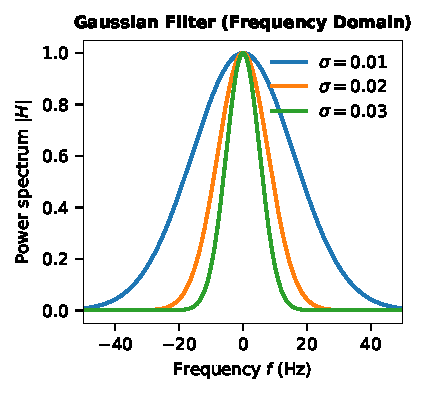
\includegraphics{media/gaussian_filters_freq.pdf}
	\caption{Gaussian low-pass filters in the time- and frequency domain. Note that the power spectrum $|H(\omega)|$ of a Gaussian filter is also a Gaussian. However, narrower (smaller $\sigma$) Gaussians in the time domain map onto broader (larger $\sigma$) Gaussians in the frequency domain.}
	\label{fig:gaussian_filters}
\end{figure}

A commonly used type of filter is the Gaussian low-pass filter (\cref{fig:gaussian_filters}). This filter is defined in the time-domain by the equation
\begin{ImportantEqn}{Gaussian Low-Pass}
	h(t) &= c^{-1} \exp\left(\frac{-t^2}{\sigma^2} \right) \,, \quad \text{where } c = \int_{-\infty}^{\infty} \exp\left(\frac{-t^2}{\sigma^2} \right) \,\mathrm{d}t \,.
\end{ImportantEqn}
The normalisation factor $c$ ensures that the overall integral over $h$ is one. This guarantees that the filter preserves the energy of a constant (\enquote{DC}) input signal.

We apply a filter to a signal using the convolution operator \enquote{$\ast$}. This operator takes two functions $f(t)$, $g(t)$ as an input and outputs a new function $(f \ast g)(t)$, where
\begin{align*}
	\big( f \ast g \big)(t) \overset{\text{def}}= \int_{-\infty}^{\infty} f(t - \tau) g(\tau) \,\mathrm{d}\tau\,.
\end{align*}

\Note{\emph{Convolution in the Fourier Domain.} It holds $\mathcal{F} [ f \ast g ] = \mathcal{F}[f] \mathcal{F}[g]$. Put differently, convolution in the time domain is simple multiplication in the frequency domain. Take another look at the frequency-space representation of the Gaussian filter in \cref{fig:gaussian_filters}.
	
Given this equation, it should be fairly obvious why this kind of filter is called a \enquote{low-pass filter} -- larger frequencies in the frequency representation of $h$ are approximately zero, multiplication with the corresponding frequency coefficients of the original signal will effectively eliminate higher frequencies from the signal. Hence the filter only passes lower frequencies on.
}

In order to use the filter for our purposes we can simply filter the individual spike trains and then multiply with the decoders 
\begin{align*}
	\hat{\vec x}(t) &= \mat D (\vec a \ast h)(t) \,.
\end{align*}
Due to linearity of the convolution operation this is equivalent to first decoding the spike trains as shown in the previous sections and then applying the filter -- which is computationally much more efficient since we only have to convolve once
\begin{ImportantEqn}{Temporal Decoding Equation}
	\hat{\vec x}(t) &= \big((\mat D \vec a) \ast h\big)(t) \,.
	\label{eqn:temporal_decoding_equation}
\end{ImportantEqn}
For a scalar signal $x(t)$ we have
\begin{align*}
	\hat{x}(t) &= \left( \left( \sum_{i = 1}^n d_i a_i \right) \ast h\right)(t) \,,
\end{align*}
where $d_i$ are the decoding coefficients and $a_i(t)$ are the individual neural activities.

\begin{figure}
	\centering
	\begin{subfigure}{\textwidth}
		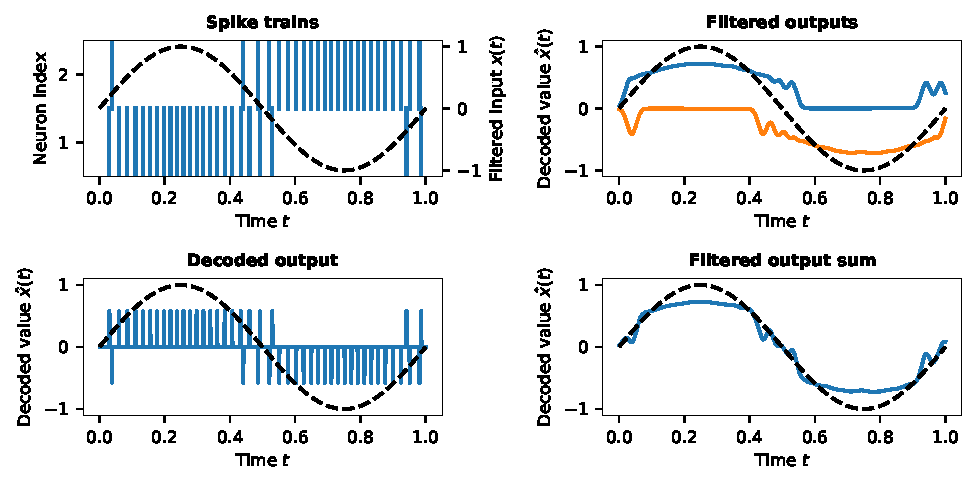
\includegraphics{media/two_neurons_filtered_small.pdf}
		\caption{Sine-wave input}
		\label{fig:two_neurons_filtered}
	\end{subfigure}
	\begin{subfigure}{\textwidth}
		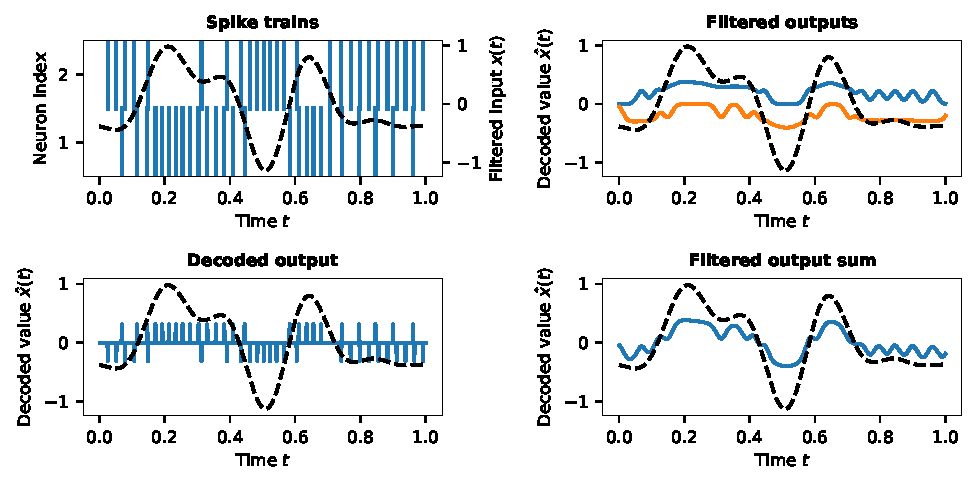
\includegraphics{media/two_neurons_filtered_white_noise_small.pdf}
		\caption{Band limited white noise input}
		\label{fig:two_neurons_filtered_white_noise}
	\end{subfigure}
	\caption{Visualisation of spike train filtering using a Gaussian filter. \textbf{(a,b)} \emph{Top left:} Spike train and input signal $x(t)$. \emph{Bottom left:} Spike trains multiplied by the corresponding decoding weights. \emph{Top right:} Individual filtered spike trains multiplied with the decoding coefficient for each neuron. \emph{Bottom right:} filtered, decoded sum of the spike trains. \CodeLink{lecture_04/filter_examples.ipynb}}
	\label{fig:filtered}
\end{figure}

As depicted in \cref{fig:two_neurons_filtered}, this technique may work quite well as long as we have control over the input signal, and we scale the output correctly. However, once we switch to a band-limited white noise input signal (\cref{fig:two_neurons_filtered_white_noise}) the error increases significantly.


\subsection{Optimal filter}

Can we do better than just using a standard Gaussian filter? Let's try to compute $h$ more systematically, for example by phrasing the filter $h$ we would like to use as the result of an optimization problem.

\paragraph{Special case: symmetric neuron tuning curves}
In order to make the mathematical derivation a little easier, let us consider the special case of a population of neurons with only two neurons, in particular the two symmetric neuron tuning curves shown in \cref{fig:two_neurons}. We generated these tuning curves by selecting exactly the same $\alpha$ and $J^\mathrm{bias}$ parameters, but choosing the encoder $e$ as $1$ for the first neuron and $-1$ for the second neuron.

Since the neurons are symmetric opposites, we can assume that $d_1 = -d_2$, i.e.,~the decoding coefficient for the second neuron is exactly the negative of the first decoding coefficient. Hence, according to \cref{eqn:temporal_decoding_equation}, we have
\begin{align*}
	\hat x(t)
		&= \big((a_1 d_1 + a_2 d_2) \ast h \big)(t) =  d_1 \big((a_1 - a_2) \ast h \big)(t) \,.
\end{align*}
Folding the scaling factor $d_1$ into $h$ we get
\begin{align*}
	\hat x(t) &= \big((a_1 - a_2) \ast h \big)(t) = \big(r \ast h \big)(t) \,,
\end{align*}
where $r(t) = a_1(t) - a_2(t)$ ($r$ for \enquote{response}). Essentially, we treat the spikes from our two neurons as being signed -- spikes from the first neuron have a positive sign, spikes from the second neuron have a negative sign.

\Note{In general, we could just use $r(t) = \langle \vec d, \vec a(t) \rangle$, although we cannot guarantee that $h$ is the optimal filter in this case (since information about the spike source is lost). For populations representing more than one dimension we can just treat the individual dimensions separately.}

\paragraph{Optimization problem}
Once again, our goal is to minimize the decoding error $\hat x(t) - x(t)$. Correspondingly, we can start with the following least-squares problem:
\begin{align*}
	h &= \arg\min_{h} E = \arg\min_{h} \int_{-\infty}^\infty \Big( x(t) - \big(r \ast h\big)(t) \Big)^2 \,\mathrm{d}t \,.
\end{align*}
Solving this equation is quite hard, since $h$ is inside an integral and a convolution operator. We can simplify this equation by switching to the Fourier domain in which convolution becomes multiplication. We have
\begin{align*}
	\hat{X}(\omega) = R(\omega)H(\omega) \,,
\end{align*}
and hence we want to find the $H$ that minimizes the error
\begin{align*}
	H &= \arg\min_{H} E = \arg\min_{H} \int_{-\infty}^{\infty} \big| X(\omega) - R(\omega) H(\omega) \big|^2 \,\mathrm{d}\omega \,.
\end{align*}
Ignoring the fact that all the objects $R(\omega)$, $H(\omega)$, $X(\omega)$ are functions, this looks quite manageable! Since this equation is quadratic in $H(\omega)$ and the second derivative with respect to $H(\omega)$ is positive, we can find the optimal $H(\omega)$ by computing the derivative and equating the result with zero. Without going into the details (see \cite{eliasmith2003neural}, Chapter 4 and Appendix B.3 for more details), we get
\begin{align*}
		H(\omega) = \frac{X(\omega) \overline{R}(\omega)}{|R(\omega)|^2} \,, \text{ where } \overline{z} = \overline{x + iy} = x - iy \text{ is the complex conjugate} \,.¸
\end{align*}
We can apply this equation to the result of a discrete Fourier transformation of $x(t)$ and $r(t)$. In this case, we can treat $X(\omega)$ and $R(\omega)$ as vectors and all operations are element-wise.

\begin{figure}
	\begin{subfigure}{\textwidth}
		\centering
		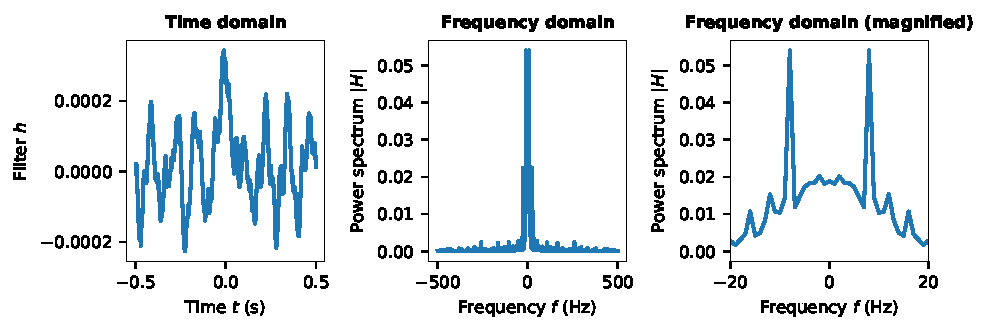
\includegraphics{media/optimal_filter.pdf}
		\caption{Optimal filter}
		\label{fig:optimal_filter}
	\end{subfigure}
	\begin{subfigure}{\textwidth}
		\centering
		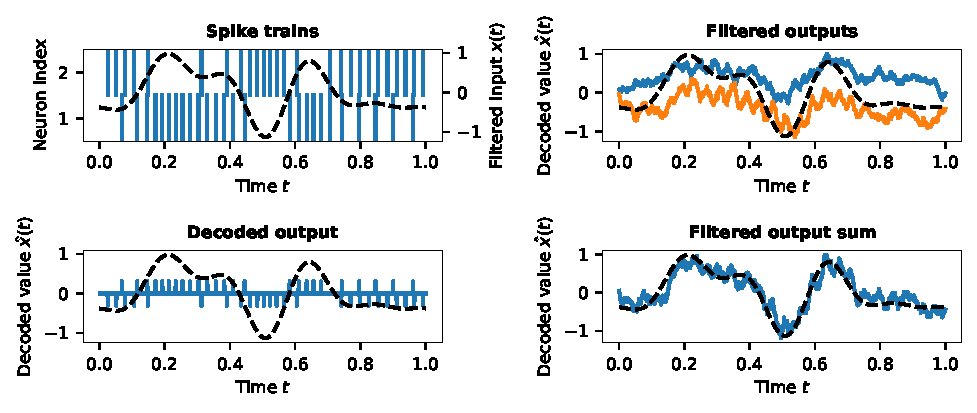
\includegraphics{media/two_neurons_filtered_optimal_simple_small.pdf}
		\caption{Spike train filtered with the optimal filter}
		\label{fig:two_neurons_filtered_optimal_simple_small}
	\end{subfigure}
	\caption{Optimal filter (top) applied to the example from \cref{fig:two_neurons_filtered_white_noise} (bottom). \CodeLink{lecture_04/filter_examples.ipynb}}
\end{figure}

\Cref{fig:optimal_filter} shows the optimal filter for a $\SI{10}{\second}$ bandlimited white noise input. This filter is then used on the input signal we already saw in \cref{fig:two_neurons_filtered_white_noise}. The result is shown in \cref{fig:two_neurons_filtered_optimal_simple_small}. Just judging visually, the error is reduced significantly. However, there is still quite some high-frequency noise present in the filtered output that is not in the original input signal. 

\paragraph{Improving the optimal filter}
Looking at the optimal filter in the frequency domain (\cref{fig:optimal_filter}), we can see the filter itself appears to be \enquote{noisy}. Could we eliminate this noise by filtering the optimal filter in the frequency domain? Doing this results in the following equation
\begin{ImportantEqn}{Optimal windowed filter}
	H(\omega)= {{(X(\omega)R^*(\omega)) \ast W(\omega)} \over {|R(\omega)|^2 \ast W(\omega)}} \,,
	\label{eqn:optimal_windowed_filter}
\end{ImportantEqn}
where $W(\omega)$ is a Gaussian filter (see above), also called a \emph{window function}. As demonstrated in \cref{fig:filter_improved}, this filter successfully eliminates the noise.

\Note{There is actually a nice mathematical derivation for \cref{eqn:optimal_windowed_filter}. Have a look at \cite{eliasmith2003neural} and Appendix B.3 for more details.}

\begin{figure}
	\begin{subfigure}{\textwidth}
		\centering
		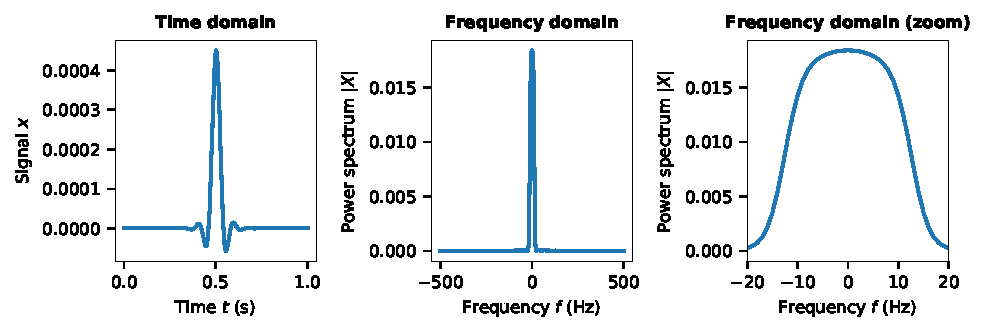
\includegraphics{media/optimal_filter_improved.pdf}
		\caption{Improved optimal filter}
		\label{fig:optimal_filter_improved}
	\end{subfigure}
	\begin{subfigure}{\textwidth}
		\centering
		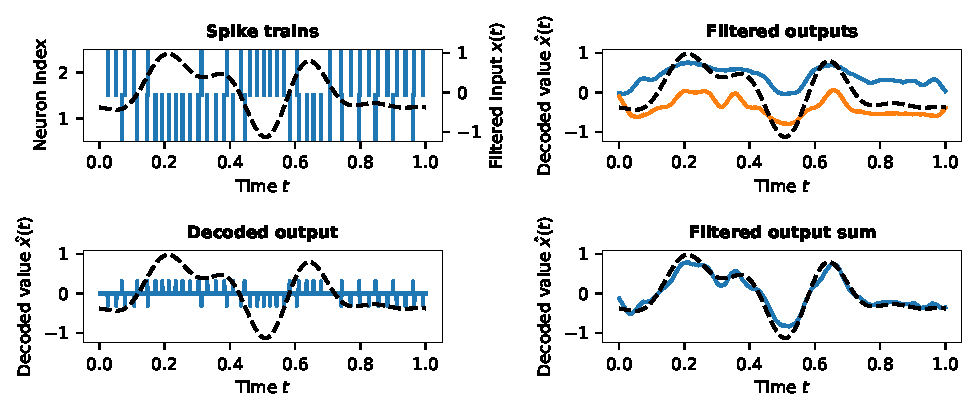
\includegraphics{media/two_neurons_filtered_optimal_small.pdf}
		\caption{Spike train filtered with the improved optimal filter}
	\end{subfigure}
	\caption{Optimal filter (top) applied to the example from \cref{fig:two_neurons_filtered_white_noise} (bottom). \CodeLink{lecture_04/filter_examples.ipynb}}
	\label{fig:filter_improved}
\end{figure}

\newpage

\section{Biological Filters}

\begin{figure}
	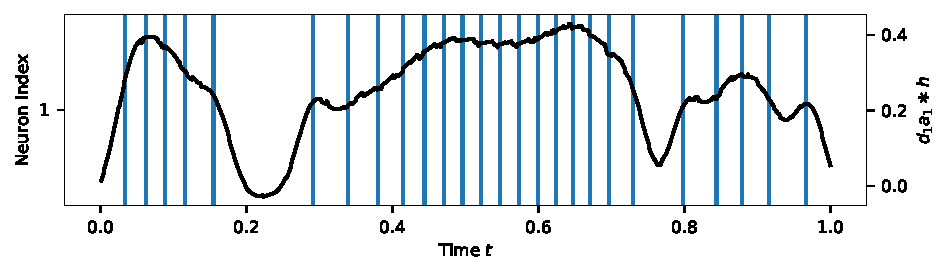
\includegraphics{media/filter_magnification.pdf}
	\caption{Optimal filter applied to the output of a single neuron. Note how future spikes influence the shape of the filtered activities.}
	\label{fig:filter_magnification}
\end{figure}

Let's have a closer look at the time-domain representation of the optimal filter depicted in \cref{fig:optimal_filter_improved}. If we think of applying this filter in terms of convolution, then this filter weighs neural activity from the past (counter intuitively, the half of the plot for $t > 0$) and neural activity from the future (the half of the plot for $t < 0$) and combines them into an estimate of the value represented by our neural population (\cref{fig:filter_magnification}). A filter that requires information about the future is called \emph{acausal}. While this is fine for analysing recorded spiking activities after the fact, this kind of filter cannot be a model of what happens inside a neurobiological system -- neurons are generally not able to look into the future.

Does this mean that we have to go back to the drawing board? Not quite. Our analysis shows that the optimal filter is essentially a low-pass filter. Hence, what we are looking for is some mechanism within a neurobiological systems that has a \enquote{smoothing} effect on the spike train. It turns out, that synapses provide this kind of filtering.

\subsection{Synaptic Filters}

\Cref{fig:synapse_schematic} once more shows a schematic drawing of a synapse. Whenever a spike arrives at the pre-synapse, synaptic vesicles fuse with the cell membrane and release neurotransmitter into the synaptic cleft. The neurotransmitter diffuses to the post-synapses, where it triggers a chemical cascade that leads to the formation of a \emph{post-synaptic potential}. Depending on the type of neurotransmitter released by the pre-synapse, this potential either has a positive, or a negative effect on the post-neuron's membrane potential. Positive potentials are called Excitatory Post-Synaptic Potential (EPSP), negative currents are called inhibitory post-synaptic potentials. The \emph{currents} causing these changes in potential are called EPSC and IPSC, respectively. \Cref{fig:burke_1967_epsp} shows such a recording of such potential in a motor neuron. As clearly visible, there is a short delay between the arrival of the pre-synaptic spike (start of the time axis), followed by a rapid increase in potential and a slow decay. This slow decay naturally acts as a low-pass filter.

\begin{figure}
	\centering
	\begin{subfigure}{0.375\textwidth}%
		\centering%
		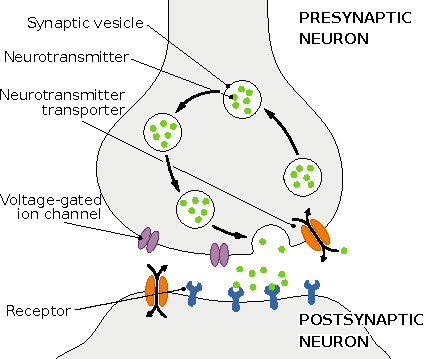
\includegraphics[width=\textwidth]{media/synapse_schematic.pdf}%
		\label{fig:synapse_schematic}
	\end{subfigure}%
	\begin{subfigure}{0.55\textwidth}%
		\centering%
		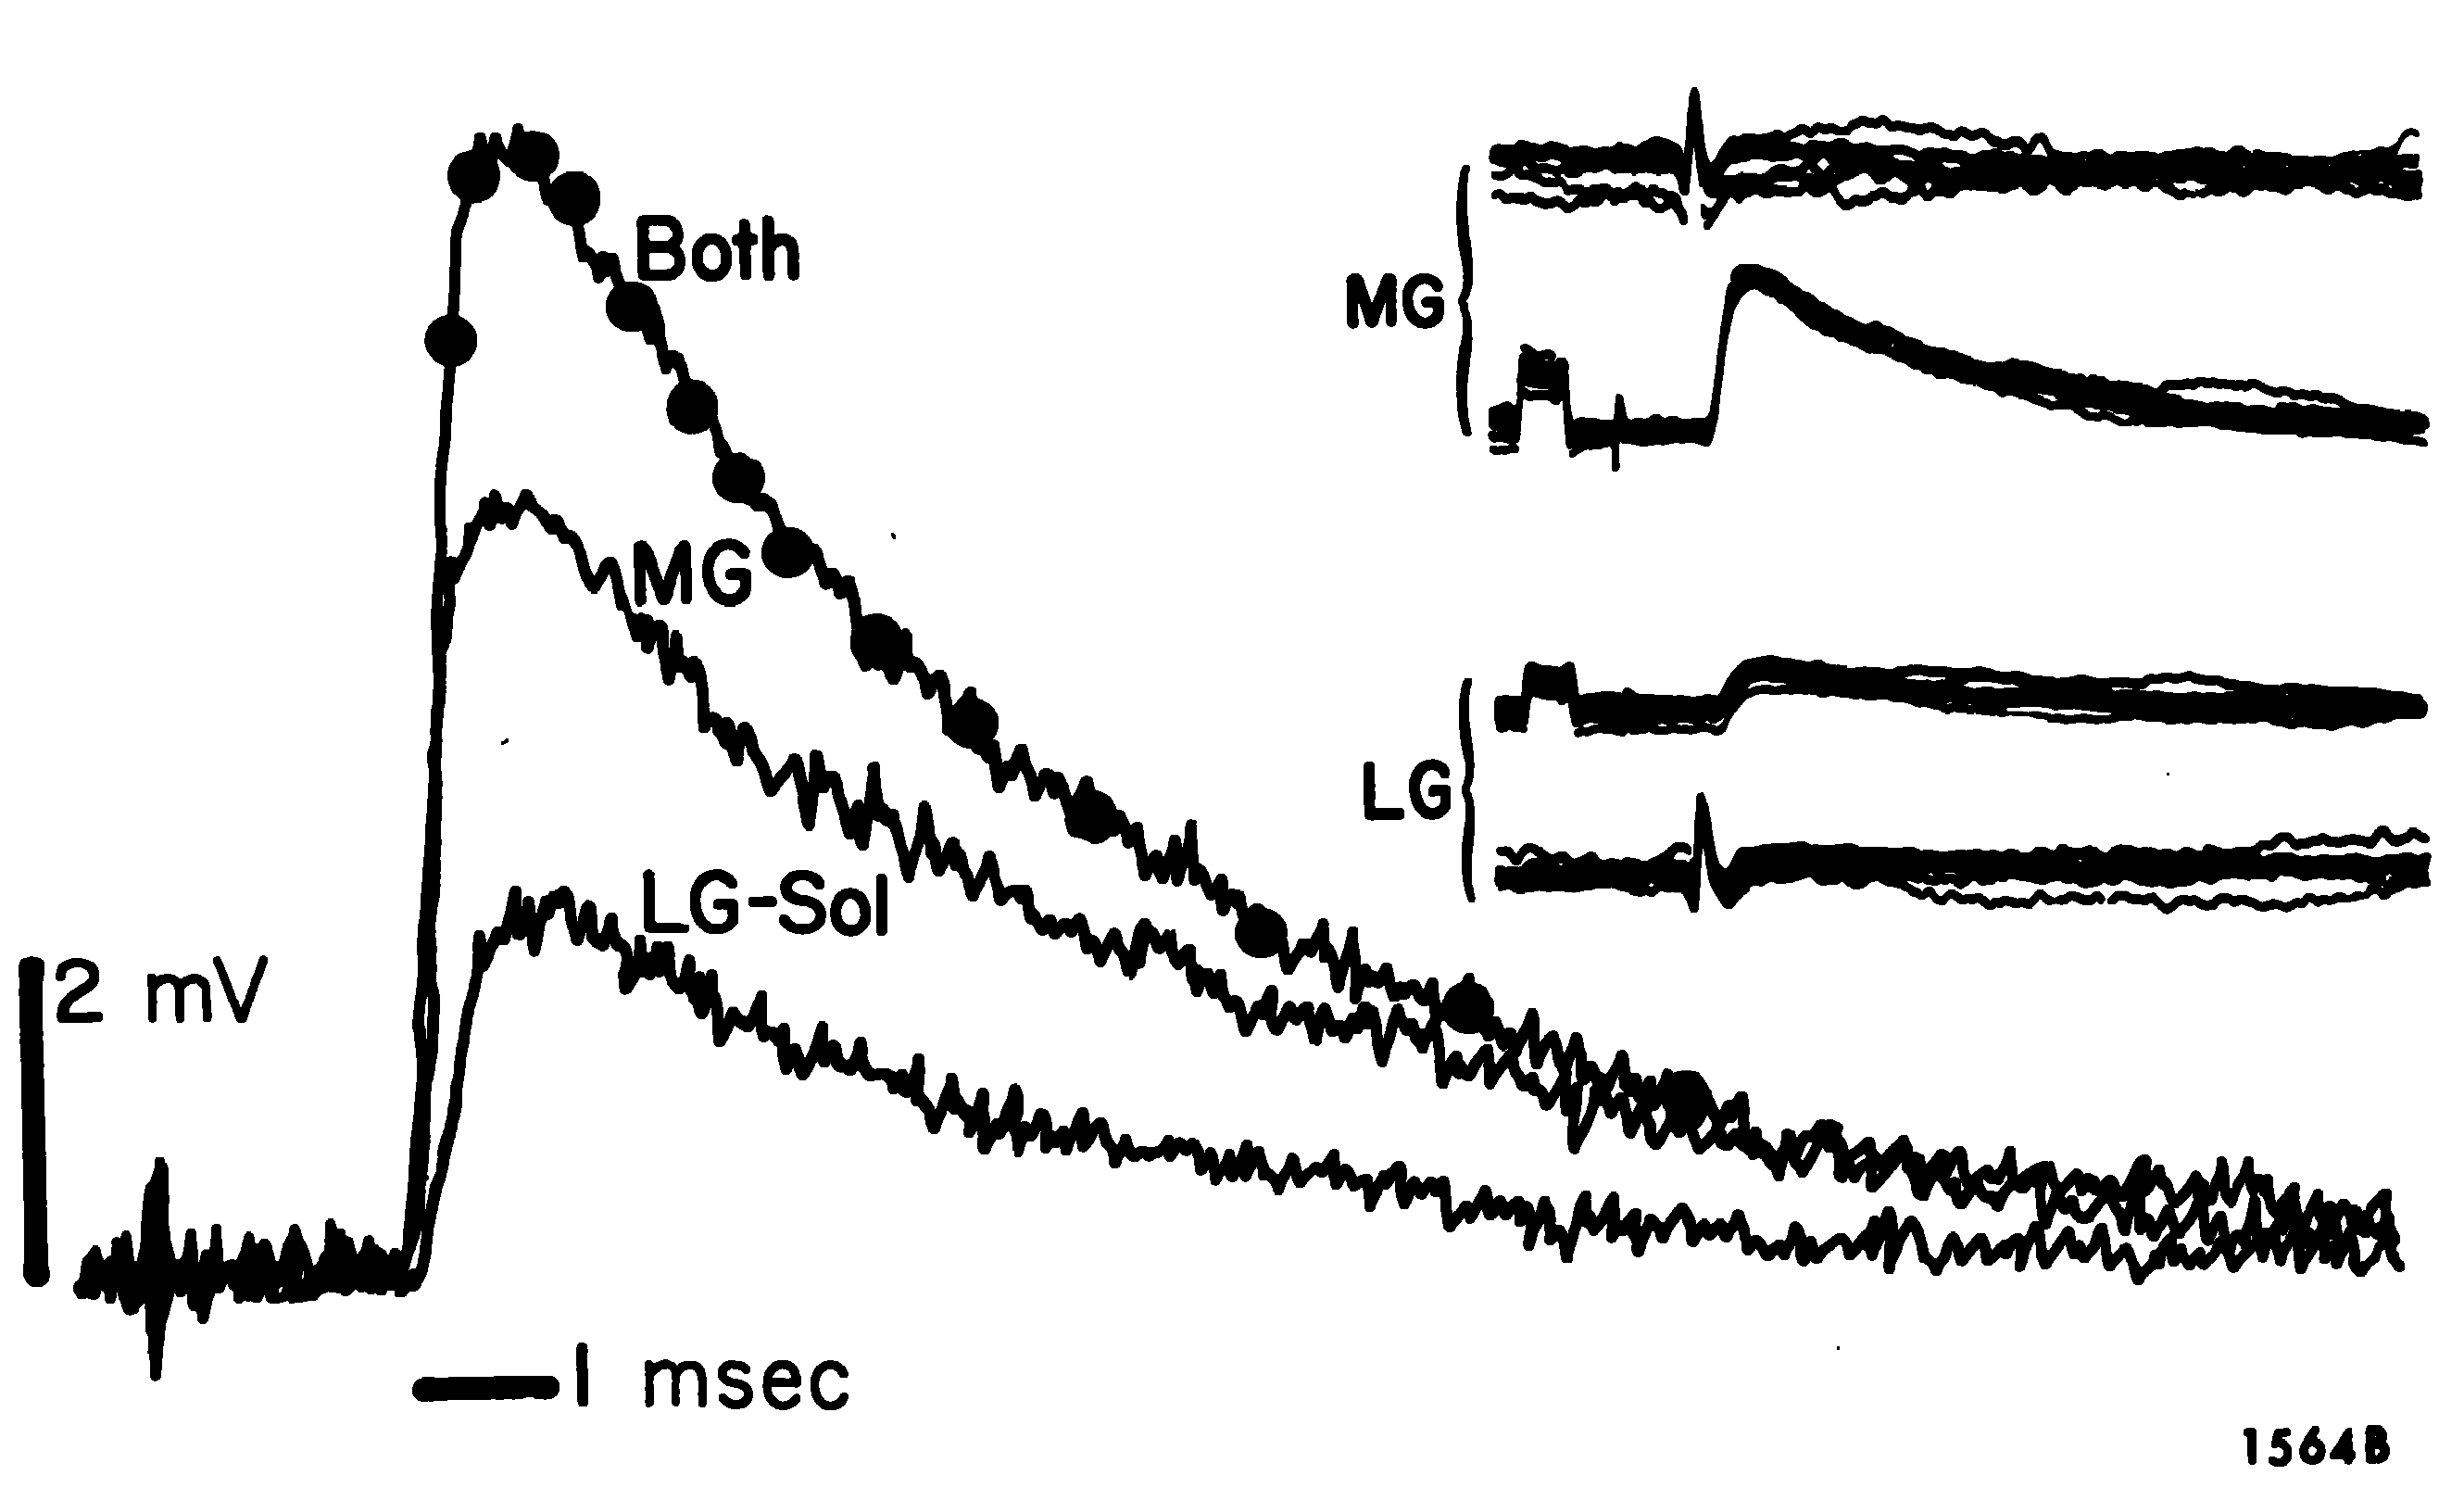
\includegraphics[width=\textwidth]{media/burke_1967_epsp.png}%
		\label{fig:burke_1967_epsp}
	\end{subfigure}%
	\caption{Synapses act as low-pass filters. \textbf{(a)} Textbook sketch of a single neuron. \textbf{(b)} Superposition of the motor potentials of two spikes arriving at a motor-neurons. Image copied from \cite{burke1967composite}.}
\end{figure}

\subsection{Models of Synaptic Filters}

Post-synaptic potentials (and the corresponding currents) are commonly modelled as a $n$-th order exponential low-pass filter. In the time domain, this filter has the following equation
\begin{ImportantEqn}{Exponential Low-Pass}
	h(t) &= \begin{cases}
		c^{-1} t^n \exp^{-t / \tau} & \text{if } t \geq 0 \,,\\
		0 & \text{otherwise}\,,
	\end{cases}
	&& \text{where } c = \int_{0}^\infty t^n \exp^{-t / \tau} \,\mathrm{d}t \,.
\end{ImportantEqn}
\Cref{fig:synaptic_filters} depicts this filter for different parameters of $n$ and $\tau$. Note how larger $\tau$ and $n$ suppresses more high-frequency content. For $n = 0$ there is a discontinuous spike onset, larger $n$ results in a smoother onset and delays the peak magnitude.

\Note{\emph{Choice of parameters.}
The parameters we use for $n$ and -- in particular -- $\tau$ depend on neurophysiological data. Descriptions of individual brain regions will often include the synaptic time constant $\tau$ and or even traces of post-synaptic responses. While there is a vast variety of time constants, inhibitory GABA-A synapses tend to have a time constant of $\tau = \SI{10}{\milli\second}$, while excitatory NMDA synapses tend to have a time constant of $\tau = \SI{5}{\milli\second}$.
}

\begin{figure}[p]
	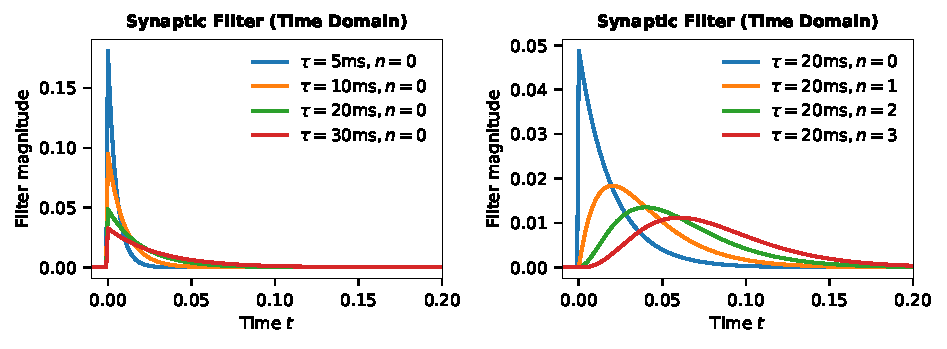
\includegraphics{media/synaptic_filters.pdf}
	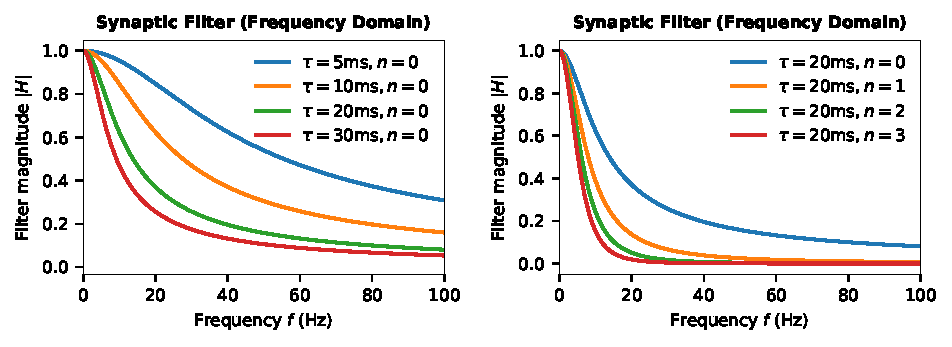
\includegraphics{media/synaptic_filters_freq.pdf}
	\caption{Exponential low-pass filters as a model of synaptic filtering. \emph{Top:} Time-domain response for different parameters $\tau$ and $n$. \emph{Bottom:} Frequency response of the corresponding filters. \CodeLink{lecture_04/media/code/filter_examples.ipynb}}
	\label{fig:synaptic_filters}
\end{figure}

\printbibliography

\end{document}
